\section{MGP-6: a controlled synthetic decision diagnostic}
\label{sec:mgp6}
MGP-6 is the name of our own memory-governance diagnostic series; it is unrelated to the third-party protocol called MGP in Section~\ref{sec:related}.
\subsection{A retained failure: MGP-6 v2}
The first version, MGP-6 v2, contained 180 scenarios, with 90 \supersede, 66 \abstain{} and 24 \keep{} items. A lookup that is fitted on the training and development splits and reads only the conflict type, without reading the dialogue or the memory state, reproduced the held-out actions exactly. Scenario recognition was therefore sufficient, and no v2 policy comparison can separate reasoning over evidence from recognition of the scenario family. A shortcut baseline that approaches the full policy is a failed construct-validity check, not a competitive result. We keep v2 as a record of the earlier instrument, and every v2 number we cite is diagnostic.

\subsection{Construction of v4.3}
MGP-6 v4.3 contains 900 items in 100 components in 20 domains, split by component into train (180 items, 20 components), development (180 items, 20 components) and hidden (540 items, 60 components). A component has nine items that share one principal, one memory slot, one standing value and one proposed value, crossed over three dialogue lengths (9, 11 and 13 turns) and three gold actions. Within a component the dialogues of all three lengths are built from the same pool of six evidence sentences, and the three actions differ in which two of the six sentences the dialogue indexes to the target slot; the three indexed pairs partition the pool. The numbering of the six sentences is also permuted between the three actions; the mean indexed position is identical for the three actions within each public split (3.600 in train, 3.575 in development, 3.5875 pooled). We verified the pool structure on the 40 public components (120 length-by-component triples). After the hidden split had already been consumed, we ran a post-hoc structural audit on all 540 hidden construction records. Using proxy components defined by principal, memory slot and standing value, the audit recovered 60 components and 180 component-by-length triples, with no parse failures; all reported Part-A structural checks passed for all 60 components and all 180 triples. The action-balance checks also passed for all 60 components, and the mean indexed position was identical across the three actions. No private component-map file was available, so equivalence between the proxy partition and an official private component map was not tested. This is a post-hoc construction check, not a performance or shortcut analysis. The model-facing record contains an opaque identifier, the stored memory (principal, slot, standing value), the dialogue and an evaluation query, and no field that names a design target or component. Items are described in the dataset card as human-authored and template-guided; we have no independent provenance for authorship.

The construction was checked against surface shortcuts by fitting word TF-IDF classifiers on 12 restricted text views, character TF-IDF classifiers on 2 views, punctuation-only and length-only features, and decision trees of depth 1 to 5 on the training split and evaluating them on the component-held-out hidden split under five seeds. Every probe stayed at or below its preset ceiling (0.40 to 0.65 depending on the view, against a chance level of 0.333); we did not recompute the per-probe accuracies and do not reproduce them here. A cross-split duplicate audit using exact hashes over seven restricted views and a character n-gram similarity threshold of 0.995 passed. Passing a ceiling does not show that no signal remains, and the checks do not show that no shortcut exists.

Two annotation packets covered all 900 items and agreed on all 900 action labels (raw agreement 1.0, kappa 1.0, 300 ambiguity flags raised); their evidence selections never matched exactly (0 of 900 items, because one packet added the first dialogue turn to every selection). Because the labelling rule is deterministic by construction, perfect agreement is consistent with the manual being followable and the items instantiating it; it does not independently validate the construct. The annotation exercise shows that the deterministic action-label manual was applied reproducibly in the two completed packets; it does not establish independent construct validity. The packets were completed by two human annotators independent of the author. The release metadata records the annotator identifiers \texttt{ALI} and \texttt{MOHAMMAD}; according to the study owner, \texttt{ALI} identifies a different individual from the author. A third independent human was designated as adjudicator according to owner-provided study metadata, but no action-label disagreement arose and the recorded label-adjudication count is zero. The builder validates records, hashes and a release attestation, but it does not authenticate reviewer identity or annotation duration.

\subsection{Evaluation protocol}
\label{sec:mgp6-protocol}
The system we call the live controller gives a language model the two messages that the public index in the dialogue points to, together with the stored memory, the requested value extracted from the dialogue, the query, and a prompt that states decision criteria for each action, and then applies a conservative guard that only changes model \abstain{} outputs when a public-evidence rule resolves them. The model was \texttt{qwen/qwen3.5-9b} through OpenRouter, with temperature 0, no reasoning, a limit of 128 new tokens and seed 4301. The configuration, including the prompt hash, was selected on the public development split and recorded in a hashed manifest before the hidden split was scored. According to the study owner, one complete hidden prediction generation was authorized for the frozen controls; it was interrupted once after 432 of 540 predictions and resumed under the same frozen controls. The hidden split has been consumed; we know of no rerun and we did not tune against it. A later successor configuration, developed on the public development split after the hidden aggregate was known (development accuracy 0.95 and 0.961 in the tracked analysis), is not part of this paper's results, and no hidden-split result for it is reported. The provider did not report the routed model revision during development, so the exact model revision behind the hosted endpoint is unknown. The hidden inputs given to the model contained no gold labels, and the run authorization required the predictions to be hashed before the private scorer was used. We omit the cost-matrix analysis that accompanies the release because its weights were committed after the hidden scoring.

\subsection{Hidden-split result}
Table~\ref{tab:hidden} gives the result for the frozen configuration. Accuracy was 0.8481 (458 of 540 items; Wilson interval 0.8154 to 0.8760). Because items within a component are not independent, we also report intervals from a bootstrap over components (60 clusters; 5\,000 resamples, seed 4301): accuracy 0.8037 to 0.8889 and macro-F1 0.8021 to 0.8894. Macro-F1 was 0.8479, Matthews correlation 0.7728 and Cohen's kappa 0.7722. No model fallbacks occurred.

\begin{table}[t]
\centering\small
\caption{Frozen live controller on the MGP-6 v4.3 hidden split (540 items, 180 per gold action). Rows are gold actions, columns are predicted actions. Precision and recall refer to the predicted or gold class respectively.}
\label{tab:hidden}
\begin{tabular}{lrrrrrr}
\toprule
Gold $\backslash$ predicted & \keep & \supersede & \abstain & Recall & Precision & F1 \\
\midrule
\keep & 151 & 11 & 18 & 0.839 & 0.795 & 0.816 \\
\supersede & 9 & 165 & 6 & 0.917 & 0.897 & 0.907 \\
\abstain & 30 & 8 & 142 & 0.789 & 0.855 & 0.821 \\
\bottomrule
\end{tabular}
\end{table}

\paragraph{Error structure.} The 38 errors on gold-\abstain{} items split into 30 predicted \keep{} and 8 predicted \supersede, a false-commit rate of 0.211 (38 of 180; Wilson interval 0.158 to 0.276), where we keep the repository's term false commit for any non-abstaining prediction on a gold-\abstain{} item; for a predicted \keep{} it does not imply that a candidate was admitted. Fifteen gold-\supersede{} items (0.083) were not superseded, and 11 gold-\keep{} items (0.061) were overwritten. Of the 374 items for which the controller did not abstain, 316 were correct (0.845), so conditional accuracy after abstention was not higher than overall accuracy (0.848); this is a descriptive statement and not evidence of calibration. A predicted \keep{} on a gold-\abstain{} item preserves the stored value; because MGP-6 v4.3 materializes no state, it counts as an error only because the gold label is \abstain{}. The guard changed 36 of the 202 model \abstain{} outputs (30 to \keep{} and 6 to \supersede).

\subsection{Development-split comparison and what it can support}
On the development split (180 items) the tracked results for \texttt{qwen/qwen3.5-9b} are summarized in Table~\ref{tab:dev}. The live controller scored 0.844 and the zero-shot policy and four structural baselines (no memory, flat retrieval, recency, naive overwrite) scored between 0.328 and 0.367. This contrast should not be read as an effect of the write policy, for two reasons that we verified in the code. First, only the live controller receives the router-extracted evidence pair; the zero-shot policy and the structural baselines receive the full public payload or a view of it. Second, the live controller also receives a different, longer prompt. The comparison therefore confounds evidence routing with the decision prompt. The four component ablations (without abstention, typing, lineage or provenance) each have their own prompt: three receive the full payload and the provenance ablation receives the dialogue without provenance, so none of them removes one component from the live controller alone.

\begin{table}[t]
\centering\small
\caption{Tracked development-split results for \texttt{qwen/qwen3.5-9b} (180 items, 60 per gold action), taken from the later complete development rerun recorded in the tracked analysis. The development run frozen before hidden scoring recorded 0.8556 accuracy (macro-F1 0.8566) for the live controller, and several baseline values differ slightly between the two runs. The live controller is the only system that receives the router-extracted evidence view.}
\label{tab:dev}
\begin{tabular}{lcc}
\toprule
System & Accuracy & Macro-F1 \\
\midrule
Live controller (with guard) & 0.844 & 0.846 \\
Decision zero-shot & 0.339 & 0.179 \\
B1 no memory & 0.367 & 0.312 \\
B2 flat retrieval & 0.356 & 0.244 \\
B3 recency & 0.328 & 0.217 \\
B4 naive overwrite & 0.339 & 0.189 \\
Ablation without abstention & 0.333 & 0.247 \\
Ablation without typing & 0.344 & 0.190 \\
Ablation without lineage & 0.350 & 0.202 \\
Ablation without provenance & 0.339 & 0.189 \\
\bottomrule
\end{tabular}
\end{table}

\paragraph{A 2 $\times$ 2 diagnostic contrast on five substitute configurations.} To see how much of this difference is associated with each of the two factors, we ran four cells on the 180 public development items: evidence view (full public payload or router-extracted pair) crossed with prompt (one-line prompt or the live-controller prompt), using the repository's own builders and temperature 0. We call the cells A (payload, one-line), D (routed, one-line), E (payload, live) and B (routed, live); B+g is cell B after the repository's guard on model \abstain{} outputs. The manuscript model was not available to us, so we used five substitute configurations of three models through a gateway (reached directly for four configurations and through a tunnel for Gemini low; the reasoning levels are gateway aliases): Gemini 3.8 Flash at low, medium and high reasoning, GLM 5.3 Flash, and gpt-oss-120b at medium reasoning. Four configurations were run twice; Gemini at high reasoning was run once. Absolute values are therefore not comparable with Table~\ref{tab:dev}, and the substitute runs do not reproduce the tracked values. The design is not a clean factorial: the prompt factor is a bundle (action definitions, resolvability criteria, abstention criteria, an instruction on the scope of the evidence and an output constraint), the system label line that the repository's prompt builder inserts is not identical across the four cells, and cell E is mismatched because the live prompt text describes two indexed messages that the full payload does not isolate. We therefore treat the experiment as a diagnostic contrast and report associated differences, not effects of the factors. Substitute models were chosen after the Gemini low accuracies had been inspected.

\paragraph{Reply parsing.} The reply parser differed among the runs, and the difference matters for the Gemini settings. We use three named rules. \emph{baseline-strict} is the repository parser at the baseline commit, which rejects a reply wrapped in a Markdown code fence. \emph{json-fence-tolerant} additionally removes one surrounding JSON fence before parsing. In the Gemini low run, our own runner extracted the text between the first and last brace; on all stored replies this gives the same action as json-fence-tolerant. GLM 5.3 Flash and gpt-oss-120b ran with the repository parser before it was modified (their runs ended before the modification time of the working copy), and their replies parse identically under both repository rules. The Gemini medium and high runs used a working copy of the repository parser that had been modified, uncommitted, to remove a JSON fence; the exact patch and hashes are in Appendix~\ref{app:parser}. The tolerant rule was introduced after fenced replies had been observed in Gemini outputs, so using it as the primary rule is a post-hoc analysis choice. We chose it because the question is which view and prompt are associated with a correct decision, not whether a model follows an output format. All accuracies below are recomputed from the stored raw replies under each rule (no stored reply exceeds the 120 characters kept, so none is truncated); a reply rejected by the parser counts as incorrect. Under baseline-strict, 49 of 1\,440, 471 of 1\,440 and 212 of 720 replies are rejected for Gemini at low, medium and high reasoning and none for the other two configurations (Appendix~\ref{app:parser}).

\paragraph{Results.} Tables~\ref{tab:models-acc}, \ref{tab:models-prompt} and~\ref{tab:models-routing} and Figure~\ref{fig:models} give the results under json-fence-tolerant. The intervals in Tables~\ref{tab:models-prompt} and~\ref{tab:models-routing} come from a paired bootstrap over the 20 components of the development split (all nine items of a component are resampled together; 10\,000 resamples, numpy \texttt{default\_rng(0)}, components indexed in order of first appearance in the development file; indices drawn with \texttt{rng.integers(0,20,(10000,20))}; one set of indices shared by all contrasts; per-item results averaged over repeats first). Item-level intervals, which ignore the clustering, differ in width (narrower for most contrasts, wider for some) and are in the supplement. We found no pattern that holds in all five configurations.
\begin{itemize}[nosep]
\item Gemini at low and medium reasoning: the live prompt was associated with higher accuracy (differences of $+0.07$ to $+0.12$; the interval excludes zero in three of four prompt contrasts), and routing with differences between $-0.01$ and $+0.03$ whose intervals include zero.
\item GLM 5.3 Flash and gpt-oss-120b: routing was associated with large gains under the one-line prompt ($+0.29$ and $+0.32$) and smaller positive gains under the live prompt ($+0.08$ and $+0.17$); the live prompt was associated with gains of $+0.24$ to $+0.28$ on the full payload and $+0.06$ to $+0.08$ on routed evidence. Each difference is smaller when the other factor is present.
\item Gemini at high reasoning (one repeat): the one-line prompt on the full payload scored 0.961, the highest cell of any configuration, and the live prompt was associated with $-0.09$ (full payload; interval $-0.16$ to $-0.03$) and $-0.07$ (routed; interval includes zero). Under the live prompt this configuration predicted \abstain{} for 84 and 81 of 180 items on the full payload and the routed pair, whereas 60 items have that gold action.
\end{itemize}
The change from cell A to cell B ranges from $-0.11$ to $+0.40$ across the five configurations under json-fence-tolerant. Under baseline-strict it is positive for all three Gemini settings ($+0.17$, $+0.40$ and $+0.31$), so the sign reversal for Gemini at high reasoning depends on the parsing rule; under baseline-strict the full-payload one-line cell of that configuration scores 0.478 and not 0.961, because 93 of its 180 replies in that cell are fenced. With the full payload and the one-line prompt, accuracy ranged from 0.34 (gpt-oss-120b, which committed a supersession for 177 of 180 items in the first repeat) to 0.96 under the tolerant rule. A statement that a full-context or one-line policy is at chance, or that the prompt or the router accounts for the development difference, therefore describes particular models and parsing rules and cannot be carried over from the manuscript model. The guard raised accuracy of cell B in all five configurations (by 0.025 to 0.050), but its separate interval includes zero in four of them.

The development split is the split on which the live prompt was selected, so cells with the live prompt may be optimistic for the manuscript model and need not transfer to other models. The gateway may add text of undocumented content to requests (reported prompt-token counts exceeded the length of our prompts by roughly 2\,000 tokens where we could compare, and for the reasoning settings the gateway's accounting may include reasoning tokens), reasoning settings differ among configurations, and the hosted model revisions are unreported. We do not extend the contrast to the hidden split or to the manuscript model, and we make no claim about which part of the prompt matters. Appendix~\ref{app:subs} lists the settings and the runs that were not used.

\begin{table}[t]
\centering\footnotesize\setlength{\tabcolsep}{4pt}
\caption{Accuracy on the 180 public development items under json-fence-tolerant parsing (mean of two repeats; one repeat for Gemini at high reasoning). A: payload, one-line prompt; D: routed pair, one-line prompt; E: payload, live prompt; B: routed pair, live prompt; B+g: B after the repository's guard. Gemini rows are Gemini 3.8 Flash at the named reasoning setting; gpt-oss-120b is at medium reasoning. Substitute models; not comparable with Table~\ref{tab:dev}.}
\label{tab:models-acc}
\begin{tabularx}{\linewidth}{lYYYYY}
\toprule
Model & A & D & E & B & B+g \\
\midrule
Gemini low & 0.761 & 0.792 & 0.881 & 0.892 & 0.928 \\
Gemini medium & 0.808 & 0.811 & 0.889 & 0.883 & 0.922 \\
Gemini high (1 repeat) & 0.961 & 0.917 & 0.867 & 0.850 & 0.900 \\
GLM 5.3 Flash & 0.503 & 0.797 & 0.783 & 0.861 & 0.889 \\
gpt-oss-120b & 0.339 & 0.658 & 0.575 & 0.742 & 0.767 \\
\bottomrule
\end{tabularx}

\end{table}

\begin{table}[t]
\centering\footnotesize\setlength{\tabcolsep}{4pt}
\caption{Prompt-associated differences in accuracy (live minus one-line prompt) with 95\% intervals from a paired bootstrap over the 20 development components. Both: routed live (B) minus payload one-line (A).}
\label{tab:models-prompt}
\begin{tabularx}{\linewidth}{lYYY}
\toprule
Model & Prompt, payload (E$-$A) & Prompt, routed (B$-$D) & Both (B$-$A) \\
\midrule
Gemini low & $+0.119$ ($0.05$, $0.19$) & $+0.100$ ($0.02$, $0.18$) & $+0.131$ ($0.04$, $0.21$) \\
Gemini medium & $+0.081$ ($0.02$, $0.14$) & $+0.072$ ($-0.01$, $0.15$) & $+0.075$ ($-0.01$, $0.15$) \\
Gemini high (1 repeat) & $-0.094$ ($-0.16$, $-0.03$) & $-0.067$ ($-0.15$, $0.02$) & $-0.111$ ($-0.19$, $-0.04$) \\
GLM 5.3 Flash & $+0.281$ ($0.22$, $0.35$) & $+0.064$ ($0.01$, $0.13$) & $+0.358$ ($0.28$, $0.43$) \\
gpt-oss-120b & $+0.236$ ($0.16$, $0.31$) & $+0.083$ ($0.01$, $0.16$) & $+0.403$ ($0.34$, $0.47$) \\
\bottomrule
\end{tabularx}

\end{table}

\begin{table}[t]
\centering\footnotesize\setlength{\tabcolsep}{4pt}
\caption{Routing-associated differences in accuracy (routed pair minus full payload) with 95\% intervals from a paired bootstrap over the 20 development components.}
\label{tab:models-routing}
\begin{tabularx}{\linewidth}{lYY}
\toprule
Model & Routing, one-line (D$-$A) & Routing, live (B$-$E) \\
\midrule
Gemini low & $+0.031$ ($-0.03$, $0.08$) & $+0.011$ ($-0.05$, $0.07$) \\
Gemini medium & $+0.003$ ($-0.06$, $0.06$) & $-0.006$ ($-0.06$, $0.05$) \\
Gemini high (1 repeat) & $-0.044$ ($-0.10$, $0.01$) & $-0.017$ ($-0.08$, $0.04$) \\
GLM 5.3 Flash & $+0.294$ ($0.22$, $0.37$) & $+0.078$ ($0.02$, $0.14$) \\
gpt-oss-120b & $+0.319$ ($0.27$, $0.37$) & $+0.167$ ($0.07$, $0.26$) \\
\bottomrule
\end{tabularx}

\end{table}

\begin{figure}[t]
\centering
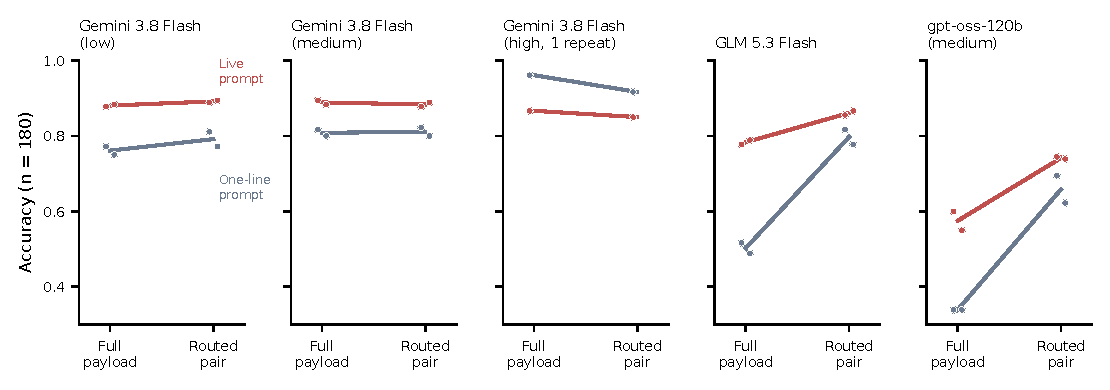
\includegraphics[width=\linewidth]{figures/fig_models.pdf}
\caption{Accuracy on the 180 public development items by evidence view and prompt for five substitute configurations of three models under json-fence-tolerant parsing (repeats shown as points, lines through the means). The sign and size of the routing-associated and prompt-associated differences depend on the configuration; see Appendix~\ref{app:parser} for baseline-strict parsing.}
\label{fig:models}
\end{figure}
